\section{Convolution}

在泛函分析中,卷积是通过两个函数$f(x)$和$g(x)$生成第三个函数的一种算子,它代表的意义是:两个函数中的一个(取$g(x)$,可以任意取)函数,把$g(x)$经过翻转平移,然后与$f(x)$的相乘,得到的一个新的函数,对这个函数积分,也就是对这个新的函数求它所围成的曲边梯形的面积。

设$f(t)$,$g(t)$是两个可积函数,$f(t)$与$g(t)$的卷积记为$f(t) * g(t)$,它是其中一个函数翻转并平移后与另一个函数乘积的积分,是一个自变量是平移量的函数。也就是:

\begin{equation}
    f(t) * g(t)=\int_{-\infty}^{+\infty} f(\tau) g(t-\tau) d \tau=\int_{-\infty}^{+\infty} f(t-\tau) g(\tau) d \tau
\end{equation}

\begin{figure}[htb!]
    \centering
    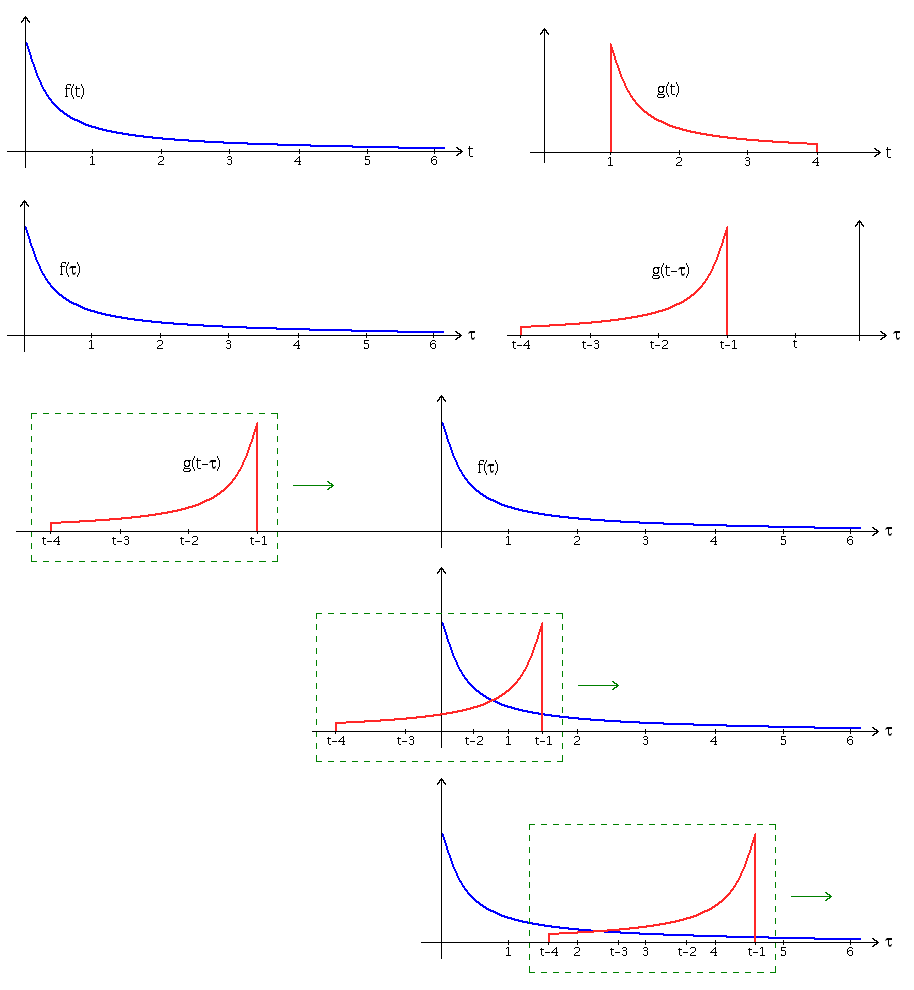
\includegraphics[scale = 0.4]{Convolution3.png}
    \caption{连续卷积图形含义}
\end{figure}

对于定义在整数$\mathbb{Z}$ 上的函数$f,g$卷积定义为:

\begin{equation}
    (f * g)(t)=\sum_{\tau=-\infty}^{\infty} f(\tau) g(t-\tau)
\end{equation}